\documentclass[conference]{IEEEtran}
\IEEEoverridecommandlockouts

\usepackage[utf8]{inputenc}
\usepackage[T1]{fontenc}
\usepackage[turkish,shorthands=:!]{babel}
\usepackage{graphicx}
\usepackage{booktabs}
\usepackage{amsmath}
\usepackage{xcolor}
\usepackage{url}
\usepackage{cite}
\usepackage[hidelinks]{hyperref}

\graphicspath{{figures/}}
\newcommand{\kod}[1]{\texttt{\small #1}}

\renewcommand{\IEEEkeywordsname}{Anahtar Kelimeler}

\begin{document}

\title{Ford Logosu Tespiti İçin Sınırlayıcı Kutu Etiketli Veri Seti Oluşturma}

\author{\IEEEauthorblockN{Ahmed Gürkan Özçelik}
\IEEEauthorblockA{Derin Öğrenme Yüksek Lisans, Öğrenci No: 250801017\\
Ostim Teknik Üniversitesi, Ankara, Türkiye\\
250801017@ostimteknik.edu.tr}}

\maketitle

\begin{abstract}
Bu çalışmada, sonraki ödevlerde nesne tespiti ve sınıflandırma modellerinin eğitiminde
kullanılmak üzere tek sınıflı (\kod{ford\_logo}) bir Ford logosu veri seti oluşturulmuştur.
Görseller \kod{icrawler} ile Bing'den üç turda toplanmış, EXIF yön düzeltmesi, RGB/JPEG
dönüşümü, 320~px alt sınırı ve algısal özet (pHash) tabanlı tekrar temizliğinden geçirilmiş,
Roboflow ile YOLO formatında etiketlenmiştir. Son veri seti 366 pozitif ve 333 negatif olmak
üzere 699 görsel ve 561 sınırlayıcı kutudan oluşur; negatiflerin tamamı benzer oval amblemler,
başka marka logolar, Ford model rozetleri ve rozetsiz araç ön yüzlerinden oluşan zor
negatiflerdir. Veri, benzer görselleri aynı bölüme toplayan grup korumalı ve tabakalı bir
yöntemle sabit tohumla (42) \%70/\%15/\%15 oranında bölünmüştür. Etiket tutarlılığı,
pozitiflerin \%10'unun körlemesine yeniden etiketlenmesiyle ölçülmüş ve ortalama IoU 0.971
bulunmuştur. Etiketler ayrıca COCO JSON formatında da sunulmuştur.
\end{abstract}

\begin{IEEEkeywords}
veri etiketleme, nesne tespiti, sınırlayıcı kutu, YOLO, COCO, veri artırma, logo tespiti
\end{IEEEkeywords}

% ---------------------------------------------------------------------------
\section{Giriş}

Derin öğrenme tabanlı nesne tespit modellerinin başarısı büyük ölçüde eğitim verisinin
niceliğine, çeşitliliğine ve etiket kalitesine bağlıdır. Yanlış ya da tutarsız etiketler
modelin öğrendiği karar sınırını bozar, test kümesine sızan tekrar görseller ise başarımın
olduğundan yüksek ölçülmesine neden olur. Bu ödevin amacı, veri hazırlama sürecinin tüm
adımlarını (toplama, temizleme, etiketleme, bölme, kayıt formatı ve kalite kontrol) uygulamalı
olarak deneyimlemek ve sonraki haftalarda hiçbir değişiklik yapılmadan PyTorch ve Ultralytics
YOLO~\cite{yolov8} eğitim kodlarına verilebilecek bir Ford logosu veri seti üretmektir.

Görsel düzeyindeki \kod{has\_logo} bilgisi sayesinde aynı veri seti logo var/yok
sınıflandırması için de kullanılabilir. Tüm adımlar betiklerle tekrarlanabilir biçimde
yapılmış ve veri seti ile birlikte \kod{scripts/} klasöründe teslim edilmiştir.

% ---------------------------------------------------------------------------
\section{Yöntem}

\subsection{Görsel toplama}

Görseller \kod{icrawler} kütüphanesinin \kod{BingImageCrawler} sınıfı~\cite{icrawler} ile
sorgu bazlı indirilmiş; her sorgu ayrı klasöre kaydedilmiş ve her görselin kaynak adresi
\kod{raw\_urls.csv} dosyasına yazılmıştır (\kod{download\_images.py}). Toplama üç turda
yapılmıştır:

\begin{enumerate}
\item \textbf{Pozitif sorgular:} ön ızgara amblemi, bagaj kapağı rozeti, gece bayi tabelası,
direksiyon logosu, anahtarlık, F-150 ön amblemi, Mustang ve Ford rozeti, eski (vintage)
rozetler. Böylece farklı bağlam, açı, ölçek ve ışık koşulları kapsanmıştır.
\item \textbf{Negatif sorgular:} Subaru, Hyundai, Toyota (benzer oval amblemler), Kia,
rozetsiz araç ızgaraları ve mavi/oval şirket logoları.
\item \textbf{Küçük logo turu} (\kod{download\_small\_logos.py}): İlk iki turdan sonra kısa
kenarı 32~px'den küçük kutu sayısı yalnızca 19'du; görsellerin çoğu yakın çekim ürün
fotoğrafıydı. Uzak mesafe tespitini desteklemek için bayi binası, otopark, yoldaki araçlar,
polis aracı ve otomobil fuarı gibi geniş açılı sahneler için 10 ek sorgu yapılmıştır. 292 ham
görselden ön işleme sonrası kalan 280 aday elle incelenmiş, logonun küçük göründüğü 50 sahne
seçilmiştir. Bu tur sonunda küçük kutu sayısı 58'e çıkmıştır.
\end{enumerate}

\subsection{Ön işleme}

Ön işleme etiketlemeden \emph{önce} uygulanmıştır (\kod{preprocess.py}):
\begin{itemize}
\item EXIF yön bilgisi \kod{PIL.ImageOps.exif\_transpose} ile görsele uygulanmış, kayıtta EXIF
yazılmayarak silinmiştir. Bu yapılmazsa bazı görseller eğitimde döndürülmüş okunur ve kutular
yanlış yere düşer.
\item Kısa kenarı 320~px'den küçük görseller elenmiştir.
\item Gri, CMYK, RGBA, PNG ve WebP dahil tüm görseller RGB'ye dönüştürülüp JPEG (kalite 95)
olarak kaydedilmiştir.
\item Tekrarlar pHash~\cite{imagehash} Hamming mesafesi $\le 4$ ile temizlenmiştir; bu
yöntem aynı görselin farklı boyutlu kopyalarını da yakalar. Yeni turlardaki görseller mevcut
tüm görsellere karşı kontrol edilmiştir.
\item Logoyu kapatan filigranlı veya aşırı bulanık görseller elle silinmiş, kalanlar
\kod{ford\_0001.jpg}, \kod{neg\_0001.jpg} biçiminde sıralı adlandırılmıştır.
\item Görseller \emph{orijinal boyutlarında} saklanmıştır; yeniden boyutlandırma ve veri
artırma eğitim sırasında yapılacaktır.
\end{itemize}

\subsection{Etiketleme aracı ve süreci}

Etiketleme Roboflow~\cite{roboflow} ile yapılmış ve YOLOv8 formatında dışa aktarılmıştır.
İlk turda Roboflow'a ön işlenmiş görseller yerine ham görseller yüklendiği için dışa aktarılan
dosya adları (\kod{000001\_jpg.rf.<hash>.jpg}) ve bazı görseller (elenmiş küçük veya tekrar
eden kopyalar) ön işlenmiş kümeyle uyuşmuyordu. Bu sorunu çözmek için
\kod{build\_dataset.py} yazılmıştır. Betik her dışa aktarılan görseli pHash ile ön işlenmiş
karşılığına eşler, en-boy oranını doğrular ve normalize YOLO kutularını orijinal boyutlu
görsele aktarır. Elenmiş görsellerin etiketleri kullanılmaz. Birden çok etiketleme turu
sırayla uygulanır ve sonraki tur öncekinin üzerine yazar. Kalite kontrolde tespit edilen
düzeltmeler de bu betikte açıkça listelenmiştir (\kod{LABEL\_OVERRIDES}), böylece tüm
düzeltmeler tekrarlanabilir.

\subsection{Etiketleme kuralları}

Yönergede verilen kurallar tüm veri setinde aynen uygulanmıştır: kutu logoya sıkı oturur;
oval görünüyorsa ovalin dış sınırı, yalnızca yazı varsa yazı kutulanır; her logo ayrı kutu ile
işaretlenir; kısmen kapanmış logoların yalnızca görünen kısmı kutulanır; yaklaşık 10~px'den
küçük ve tanınamayan logolar etiketlenmez; yansıma ve ekran/poster üzerindeki tanınabilir
logolar etiketlenir; negatiflerde boş etiket dosyası bulunur. Kuralların kapsamadığı durumlar
için alınan özel kararlar şunlardır:

\begin{enumerate}
\item \textbf{Oval içinde ikinci kutu yok.} Oval görünüyorsa içindeki ``Ford'' yazısı ayrıca
kutulanmaz. İlk turda bu kurala uymayan iç kutular, başka bir kutunun \%95'inden fazlası içinde
kalan ve alan oranı 0.15--0.6 olan kutuları silen bir kuralla otomatik temizlenmiştir.
\item \textbf{Model rozetleri Ford logosu değildir.} Mustang atı, F-150, Raptor, ST ve Focus
rozetleri kutulanmaz; başka Ford logosu yoksa görsel zor negatiftir.
\item \textbf{Büyük harfli ``FORD'' yazısı} (tabela harfleri, eski arma üzerindeki yazı,
bagaj kapağı harfleri) logo kabul edilir ve yalnızca yazı kutulanır.
\item \textbf{Yazısız boş oval} kapak etiketlenmez.
\item \textbf{Logo ızgaraları} (çok sayıda şirket logosu) içindeki Ford logosu 10~px sınırını
geçiyorsa etiketlenir.
\item \textbf{Üst üste dizilmiş amblemler} görünen kısımları kadar ayrı ayrı kutulanır.
\item \textbf{Stok fotoğraf filigranları} logoyu kapatmıyorsa görsel tutulmuştur.
\item \textbf{10~px sınırı:} Kısa kenarı 8--9~px olup biçimi ve konumu sayesinde açıkça
tanınan 5 kutu etiketlenmiştir.
\item \textbf{Örnek görseller ile yazılı kural farkı:} Yönergedeki örnek görsellerde kutu
ovalin içindeki yazıyı kapsarken yazılı kural ovalin dış sınırını tarif etmektedir.
Tutarlılık için tek bir tanım seçilmiş ve ölçülebilir olduğu için yazılı kural uygulanmıştır.
\end{enumerate}

\subsection{Eğitim/doğrulama/test bölmesi}

Bölme \kod{split.py} ile sabit tohum (\kod{seed=42}) kullanılarak \%70/\%15/\%15 oranında
yapılmıştır. Pozitif ve negatifler ayrı ayrı bölünerek oran her bölümde korunmuştur
(pozitif oranı train/val/test: 0.52/0.53/0.52). Aynı fotoğraf serisinden kareler veya aynı
sahnenin farklı ajanslardaki kopyaları gibi çok benzer görseller, pHash mesafesi $\le 10$ olan
çiftleri birleştiren bir union-find yapısıyla gruplanmış ve her grup bütün olarak tek bir
bölüme atanmıştır. 699 görsel 672 gruba ayrılmış, 19 grup birden fazla görsel içermiştir.
Gruplar büyükten küçüğe, hedefe göre en çok eksiği olan bölüme yerleştirilmiştir. Bu bölme
sonraki ödevlerde değiştirilmeden kullanılacaktır.

\subsection{Kayıt formatı}

Veri seti yönergedeki klasör yapısına uygundur: \kod{images/\{train,val,test\}},
aynı adlı etiket dosyalarıyla \kod{labels/\{train,val,test\}}, \kod{data.yaml},
\kod{classes.txt}, \kod{metadata.csv}, \kod{README.md}, \kod{scripts/} ve
\kod{augmentation\_ornekleri/}. YOLO etiketlerinde her satır
\kod{<sınıf> <x\_merkez> <y\_merkez> <genişlik> <yükseklik>} biçimindedir; değerler görsel
boyutuna bölünerek 0--1 aralığına normalize edilir ve 6 ondalık basamakla yazılır.
\kod{metadata.csv} her görsel için bölüm, \kod{has\_logo}, kutu sayısı, boyut, kaynak URL ve
not (ör. ``zor negatif -- benzer oval logo (Subaru)'') bilgisini içerir.

Ek puan kapsamında etiketler COCO~\cite{coco} formatında da dışa aktarılmıştır
(\kod{annotations/instances\_\{train,val,test\}.json}). İki format arasındaki farklar
Tablo~\ref{tab:format}'de özetlenmiştir. Dönüşüm
$x_{\text{sol}} = (x_c - w/2)\,W$, $w_{\text{px}} = w\,W$ (y ve h için $H$ ile) şeklindedir.

\begin{table}[t]
\centering
\caption{YOLO ve COCO formatlarının karşılaştırılması}
\label{tab:format}
\begin{tabular}{@{}lll@{}}
\toprule
 & YOLO & COCO \\
\midrule
Dosya & görsel başına \kod{.txt} & bölüm başına \kod{.json} \\
Kutu & $x_c, y_c, w, h$ (merkez) & $x, y, w, h$ (sol üst) \\
Birim & normalize (0--1) & piksel \\
Sınıf no & 0'dan başlar & \kod{category\_id} 1'den \\
Negatif & boş \kod{.txt} & anotasyonsuz görsel \\
\bottomrule
\end{tabular}
\end{table}

\subsection{Kalite kontrol}

\begin{itemize}
\item \textbf{Doğrulama betiği:} Ders kapsamında resmî bir \kod{check\_dataset.py}
paylaşılmadığı için yönergede listelenen tüm kontroller bu adla yazılmıştır: klasör yapısı,
\kod{data.yaml} ve \kod{classes.txt} içeriği, her görselin etiket dosyası (ve tersi), dosya adı
biçimi, JPEG/RGB/EXIF/320~px, satır başına 5 değer, sınıf no, 0--1 aralığı ve kutunun görsel
dışına taşmaması, negatif/pozitif etiket tutarlılığı, aynı dosyanın (ad veya MD5 içerik
özeti) birden fazla bölümde bulunmaması ve \kod{metadata.csv}'nin dosyalarla tutarlılığı.
Betiğin hataları gerçekten yakaladığı, bilerek bozulmuş bir kopya üzerinde 7 farklı hata
türüyle doğrulanmıştır. Teslim edilen veri seti \textbf{0 hata} ile geçmektedir; 5 uyarı
özel karar 8'deki küçük kutulardır.
\item \textbf{Görsel kontrol:} \kod{visualize\_labels.py} ile 40 rastgele görselin kutuları
çizilmiş (Şekil~\ref{fig:qc}), ayrıca tüm pozitifler pano halinde gözden geçirilmiştir.
\item \textbf{Yeniden etiketleme:} Pozitiflerin \%10'u eski kutular görülmeden ayrı bir
Roboflow projesinde yeniden etiketlenmiş ve \kod{relabel\_check.py} ile karşılaştırılmıştır
(Bölüm~\ref{sec:relabel}).
\end{itemize}

Kalite kontrolde bulunan ve düzeltilen başlıca hatalar şunlardır: negatif klasöründe Ford
logosu içeren 15 görsel (logo ızgaraları, bayi tabelaları) etiketlenip pozitife aktarılmıştır;
yalnızca model rozeti içeren 98 ``pozitif'' görsel zor negatife aktarılmıştır; oval içi ikinci
kutular silinmiştir; 15 eski arma görselinde tüm armayı kapsayan kutular özel karar 3'e göre
yalnızca yazıyı kapsayacak şekilde yeniden çizilmiştir.

% ---------------------------------------------------------------------------
\section{Veri Seti İstatistikleri}

Bölüm bazında dağılım Tablo~\ref{tab:split}'de verilmiştir. Pozitif görsellerin \%81'inde
tek kutu bulunurken bazı ürün ve logo ızgarası görsellerinde 24'e kadar kutu vardır
(Şekil~\ref{fig:stats}b). Kutu alanının görsel alanına oranı log ölçekte geniş bir aralığa
yayılmıştır (medyan \%4.8, en küçük \%0.01); küçük logo turuyla dağılımın sol kuyruğu
belirgin biçimde güçlenmiştir (Şekil~\ref{fig:stats}c). Görsel çözünürlükleri
369--5472~px genişlik ve 320--6000~px yükseklik arasındadır, medyan 1140$\times$956'dır
(Şekil~\ref{fig:stats}d).

\begin{table}[t]
\centering
\caption{Bölüm bazında görsel ve kutu sayıları}
\label{tab:split}
\begin{tabular}{@{}lrrrrr@{}}
\toprule
Bölüm & Görsel & Pozitif & Negatif & Kutu & Oran \\
\midrule
train & 489 & 255 & 234 & 377 & \%70.0 \\
val   & 105 &  56 &  49 &  91 & \%15.0 \\
test  & 105 &  55 &  50 &  93 & \%15.0 \\
\midrule
Toplam & 699 & 366 & 333 & 561 & \\
\bottomrule
\end{tabular}
\end{table}

\begin{figure}[t]
\centering
\begin{tabular}{@{}c@{\hspace{2pt}}c@{}}
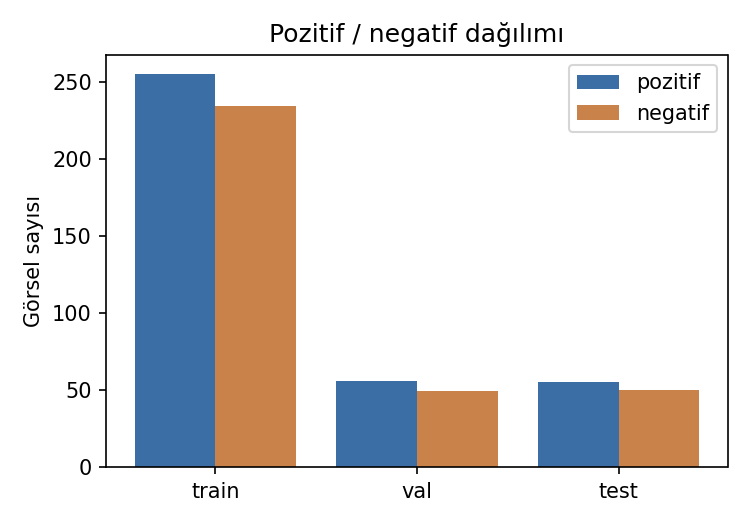
\includegraphics[width=0.49\columnwidth]{pozitif_negatif.png} &
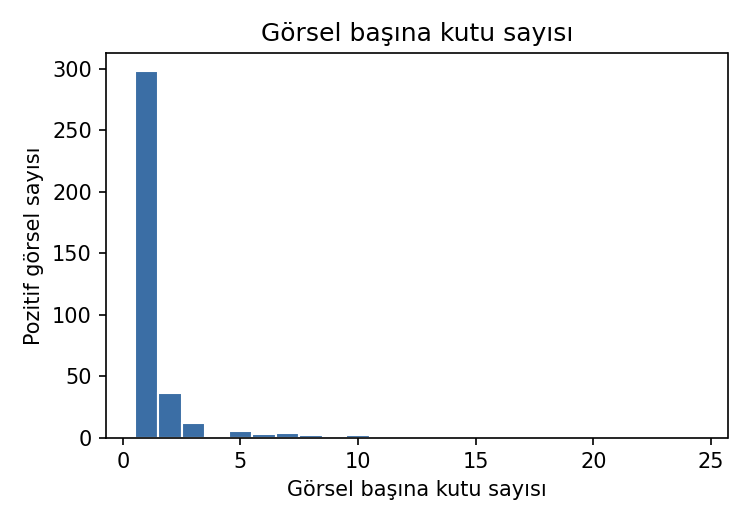
\includegraphics[width=0.49\columnwidth]{kutu_sayisi.png} \\
\small (a) & \small (b) \\
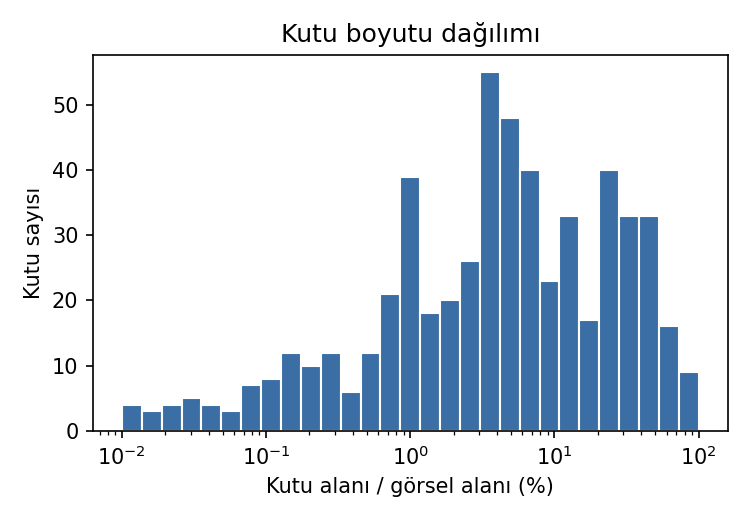
\includegraphics[width=0.49\columnwidth]{kutu_boyutu.png} &
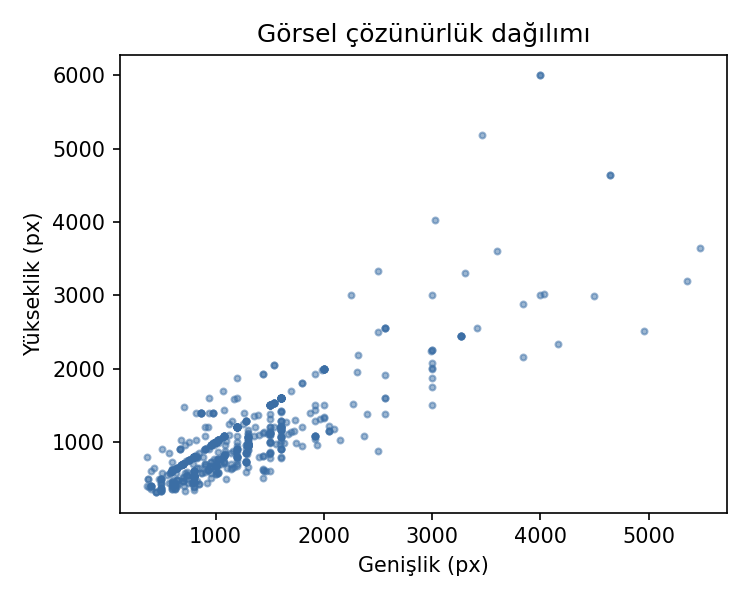
\includegraphics[width=0.49\columnwidth]{cozunurluk.png} \\
\small (c) & \small (d)
\end{tabular}
\caption{(a) Bölüm bazında pozitif/negatif dağılımı, (b) görsel başına kutu sayısı,
(c) kutu alanı/görsel alanı (log ölçek), (d) görsel çözünürlüğü.}
\label{fig:stats}
\end{figure}

Normalizasyon için kanal bazında ortalama ve standart sapma yalnızca \textbf{train}
kümesinin 835 milyon pikselinden hesaplanmıştır; doğrulama ve test bilgisi modele sızmasın
diye diğer bölümler kullanılmamıştır:
\begin{equation*}
\mu = [0.4822,\ 0.4749,\ 0.4899],\quad \sigma = [0.3474,\ 0.3452,\ 0.3410].
\end{equation*}

Zor negatiflerin dağılımı: 98 Ford model rozeti (Mustang atı, F-150, Raptor, ST), 87 başka
marka oval amblem (Hyundai, Toyota), 69 benzer oval/mavi logo (Subaru, şirket logoları),
40 başka marka amblem (Kia) ve 39 rozetsiz araç ön yüzü.

% ---------------------------------------------------------------------------
\section{Örnek Görseller ve Ek Denemeler}

Şekil~\ref{fig:examples} farklı bağlamlardan etiketli örnekleri, Şekil~\ref{fig:neg} zor
negatif örneklerini, Şekil~\ref{fig:small} ise küçük logo turundan büyütülmüş kesitlerle
örnekleri göstermektedir.

\textbf{Letterbox denemesi.} Görseller ayrı bir deneme olarak oran korunarak
224$\times$224'e yeniden boyutlandırılmış ve boşluklar gri (114) ile doldurulmuştur
(\kod{letterbox\_demo.py}). Ölçek $r=\min(224/W,\,224/H)$, dolgu
$d_x=\lfloor(224-\mathrm{round}(Wr))/2\rfloor$ olmak üzere kutular
$x_c' = (x_c W r + d_x)/224$, $w' = w W r/224$ dönüşümüyle güncellenmiştir (y ekseni için
benzer şekilde). Şekil~\ref{fig:letterbox} kutuların dönüşümden sonra da logoya oturduğunu
göstermektedir.

\textbf{Veri artırma.} Albumentations~\cite{albumentations} ile yatay çevirme, $\pm15^\circ$
döndürme, parlaklık/kontrast, ölçekleme, kutuyu koruyan rastgele kırpma, renk tonu, bulanıklık
ve bunların birleşimi uygulanmıştır. Kutular görselle birlikte dönüştürülmüştür
(Şekil~\ref{fig:aug}). Bu görseller yalnızca rapor içindir ve veri sızıntısını önlemek için
train/val/test klasörlerine eklenmemiştir.

\begin{figure*}[t]
\centering
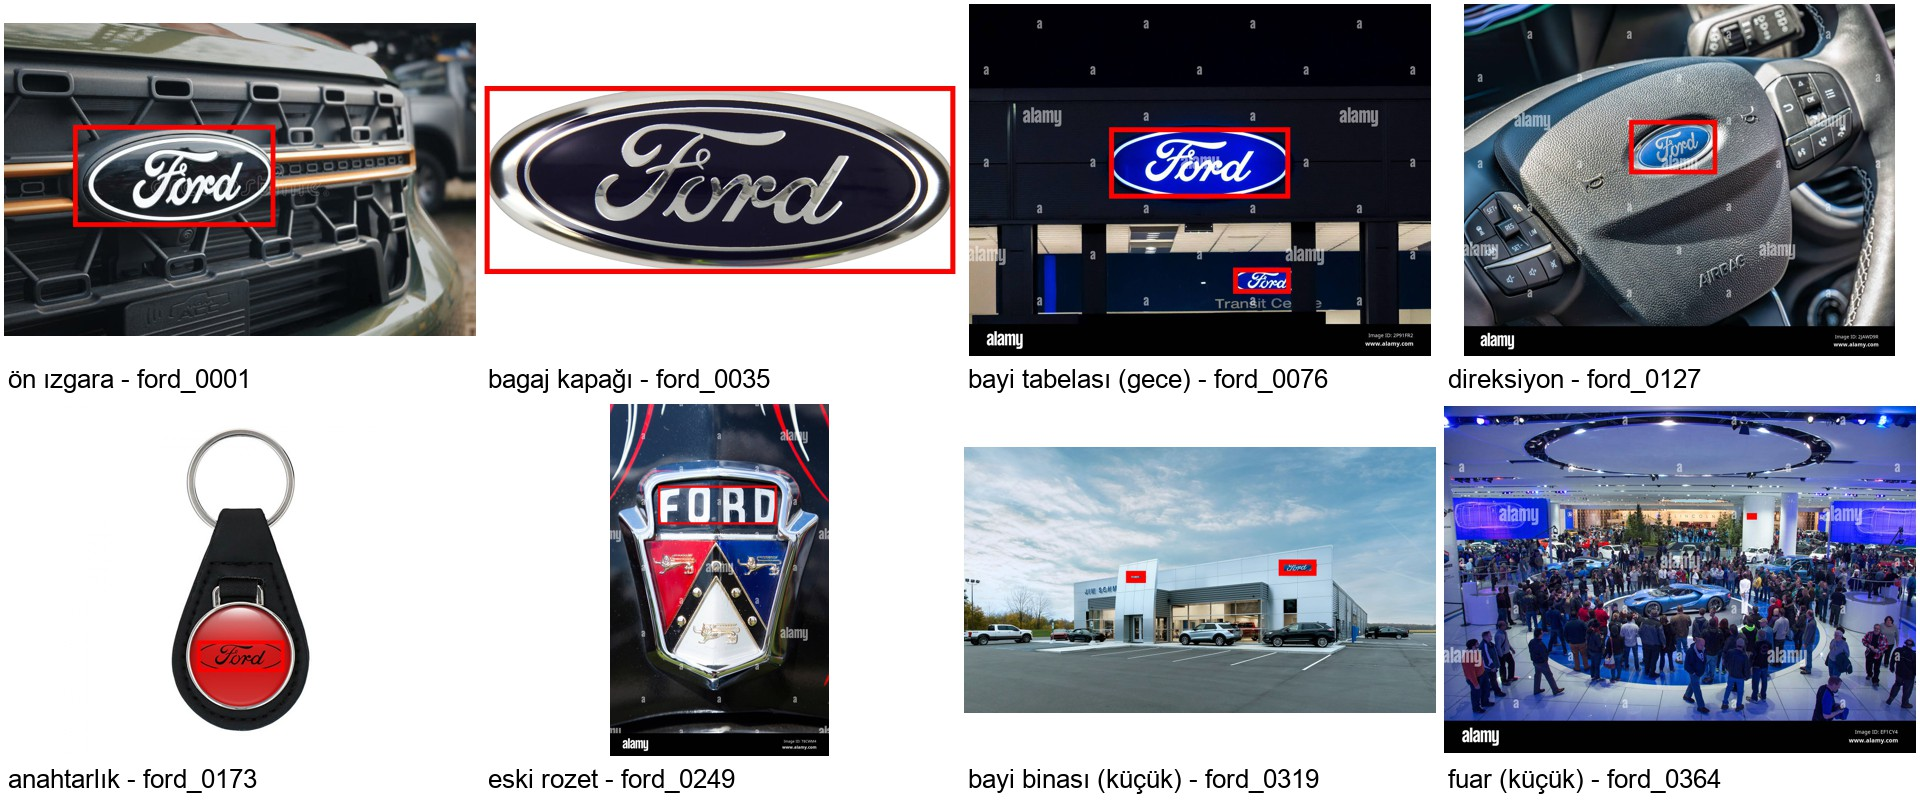
\includegraphics[width=\textwidth]{ornekler.jpg}
\caption{Farklı bağlamlardan etiketli örnekler (kırmızı: sınırlayıcı kutu). Alt satırdaki
son iki görsel küçük logo turundandır.}
\label{fig:examples}
\end{figure*}

\begin{figure*}[t]
\centering
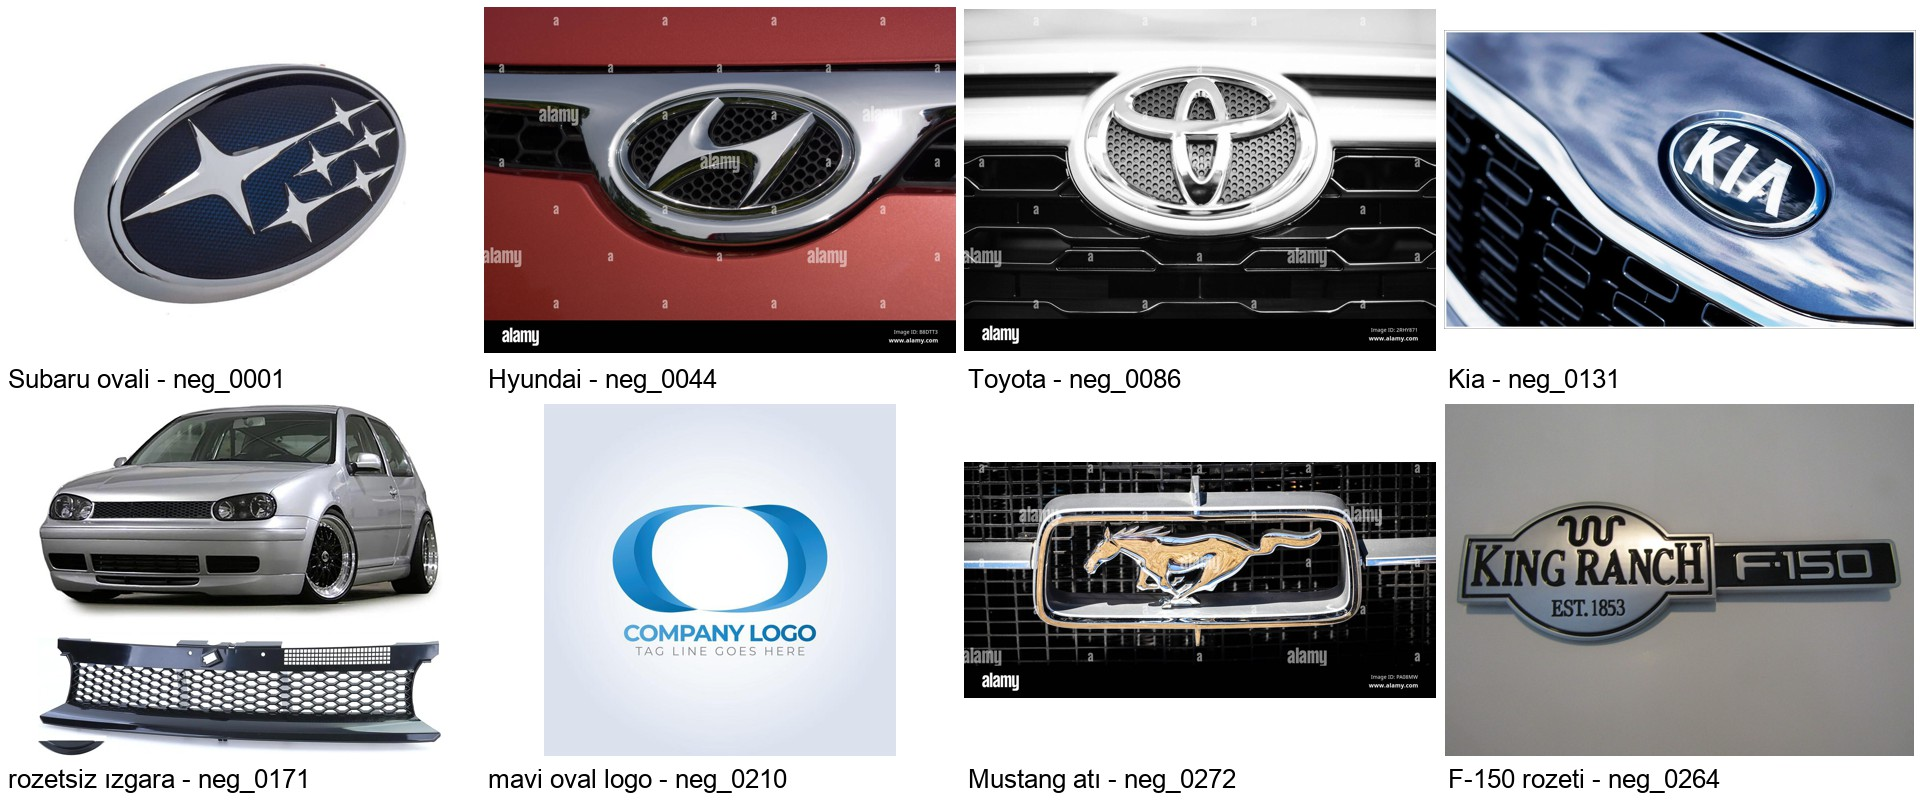
\includegraphics[width=\textwidth]{zor_negatifler.jpg}
\caption{Zor negatif örnekleri: benzer oval amblemler, başka marka logolar, rozetsiz ızgara ve
Ford logosu sayılmayan model rozetleri (Mustang atı, F-150).}
\label{fig:neg}
\end{figure*}

\begin{figure}[t]
\centering
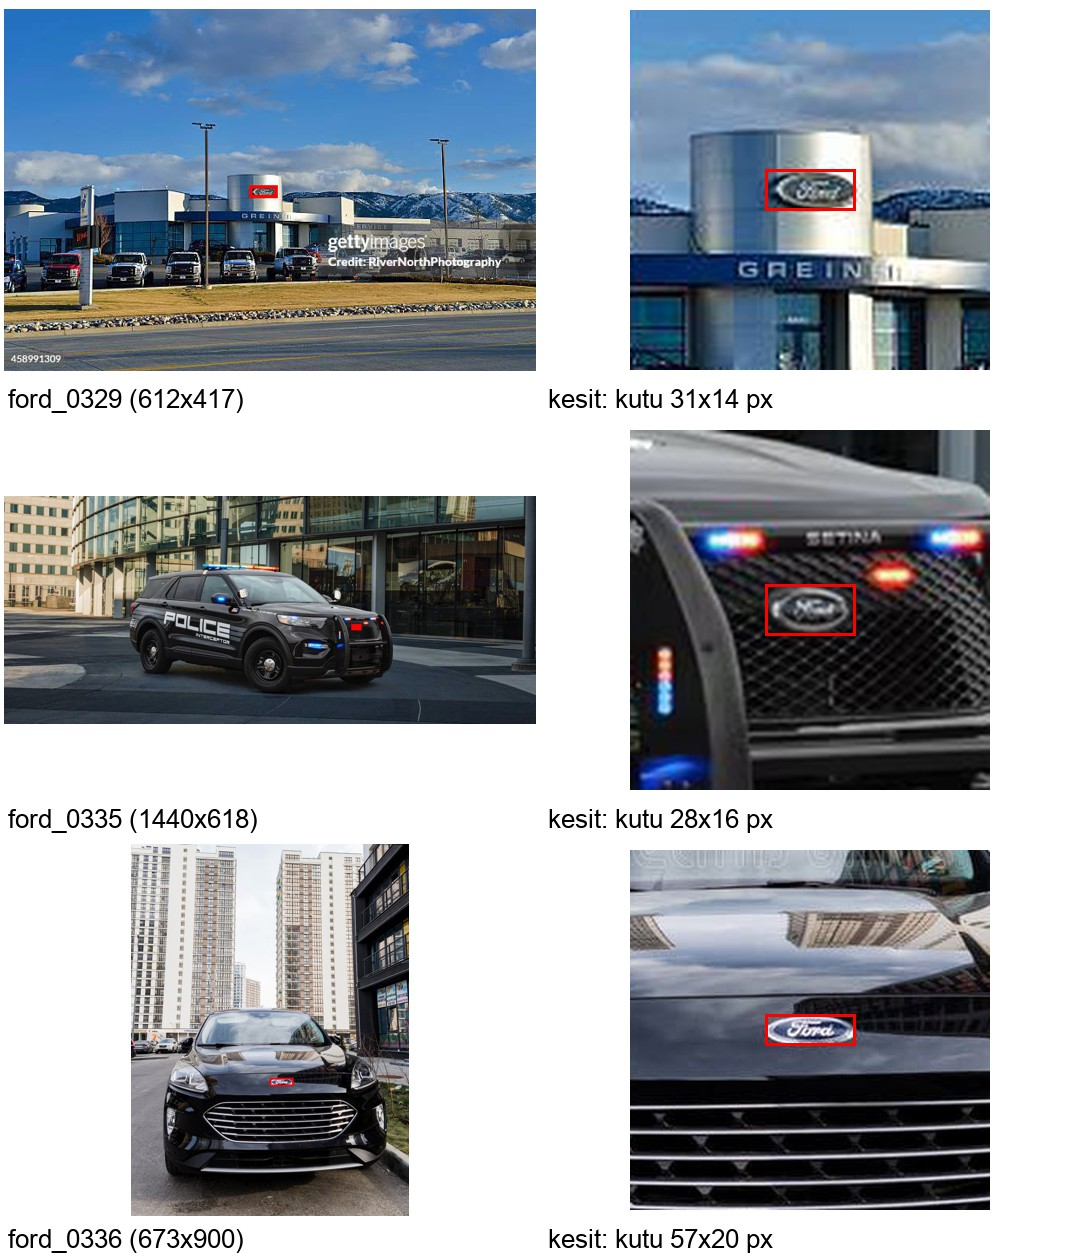
\includegraphics[width=\columnwidth]{kucuk_logolar.jpg}
\caption{Küçük logo örnekleri. Sol: tam görsel, sağ: kutu çevresinden büyütülmüş kesit.}
\label{fig:small}
\end{figure}

\begin{figure}[t]
\centering
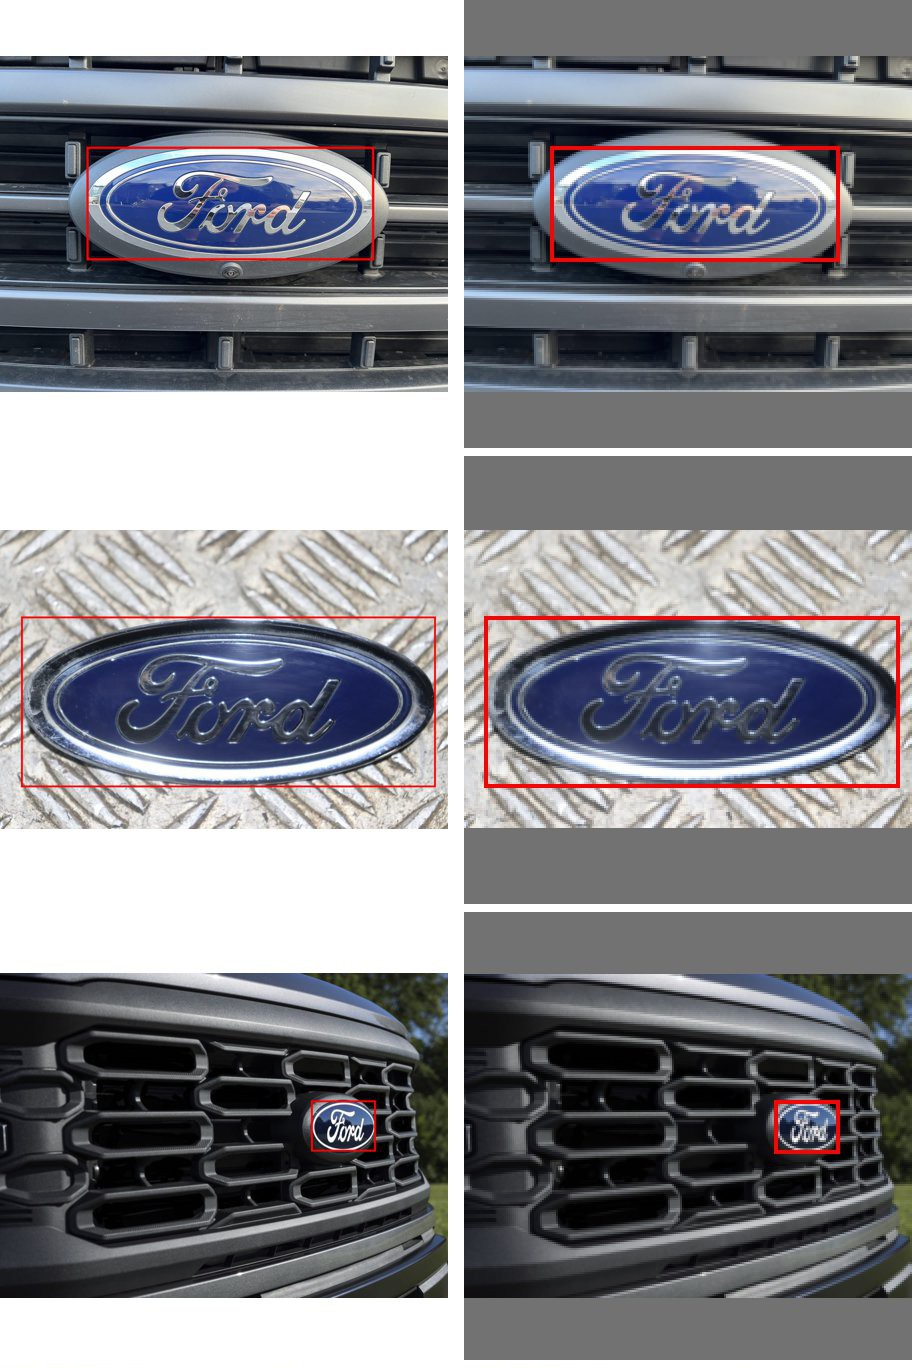
\includegraphics[width=0.8\columnwidth]{letterbox.jpg}
\caption{Letterbox denemesi. Sol: orijinal görsel ve kutu, sağ: 224$\times$224 letterbox
sonrası dönüştürülmüş kutu.}
\label{fig:letterbox}
\end{figure}

\begin{figure}[t]
\centering
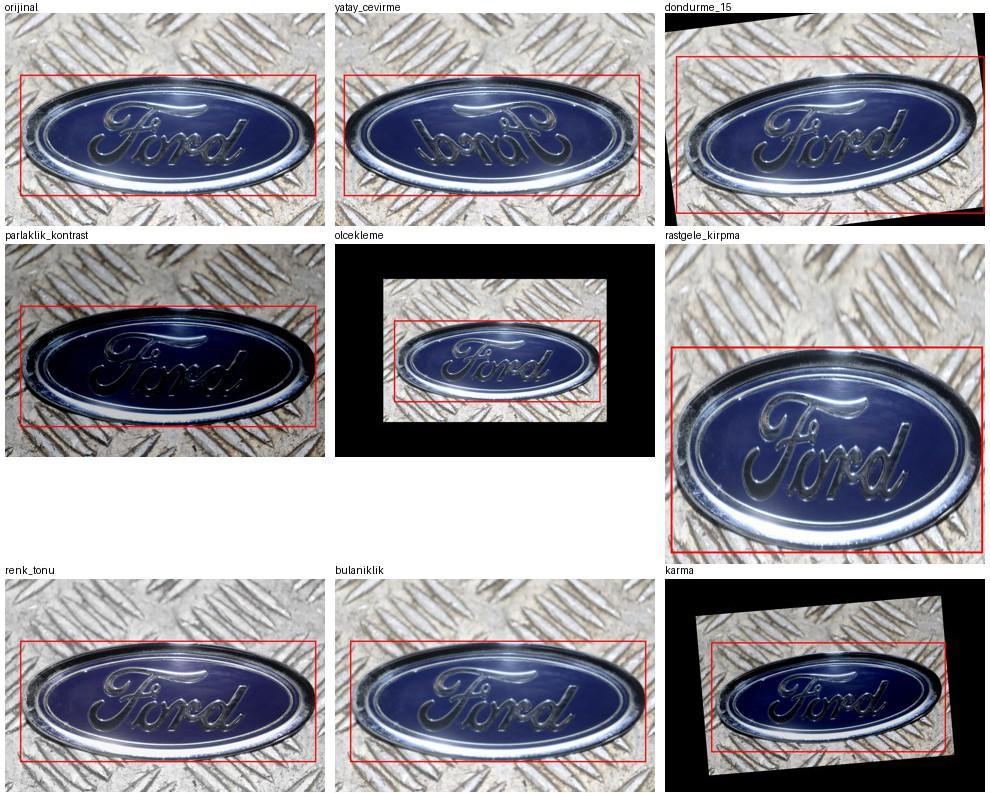
\includegraphics[width=\columnwidth]{augmentation.jpg}
\caption{Kutularla birlikte dönüştürülmüş veri artırma örnekleri.}
\label{fig:aug}
\end{figure}

% ---------------------------------------------------------------------------
\section{Yeniden Etiketleme ile Tutarlılık Ölçümü}
\label{sec:relabel}

Pozitiflerden önce 32 görsel rastgele seçilmiş (seed 42), küçük logo turu pozitif sayısını
366'ya çıkarınca oranı korumak için yeni turdan 5 görsel daha eklenmiştir (toplam
37/366~=~\%10.1). Görseller eski kutular görülmeden ayrı bir Roboflow projesinde yeniden
etiketlenmiş ve iki etiketleme açgözlü IoU eşleştirmesiyle karşılaştırılmıştır
(Tablo~\ref{tab:relabel}).

\begin{table}[t]
\centering
\caption{Yeniden etiketleme sonuçları (düzeltme öncesi)}
\label{tab:relabel}
\begin{tabular}{@{}lrrr@{}}
\toprule
Ölçüt & İlk örnek & Ek örnek & Toplam \\
\midrule
Görsel & 32 & 5 & 37 \\
İlk etiketlemedeki kutu & 49 & 8 & 57 \\
Eşleşen kutu (IoU $>$ 0.1) & 48 & 7 & 55 \\
Ortalama IoU & 0.976 & 0.937 & 0.971 \\
IoU $\geq$ 0.75 oranı & \%100 & \%100 & \%100 \\
Tutarsız görsel & 1 & 1 & 2 \\
\bottomrule
\end{tabular}
\end{table}

İki tutarsızlık bulunmuştur (Şekil~\ref{fig:relabel}):
\begin{enumerate}
\item \kod{ford\_0252} (eski arma): İlk etiketleme tüm armayı, ikinci etiketleme yalnızca
``FORD'' yazısını kapsıyordu (IoU 0.07). Özel karar 3'e göre ikinci etiket doğrudur. Bu
bulgu üzerine 56 eski arma görselinin tamamı taranmış, aynı hatayı içeren 15 görsel
yeniden etiketlenerek yalnızca yazı kutulanmıştır.
\item \kod{ford\_0366} (otomobil fuarı): İkinci etiketlemede arkadan aydınlatılmış, düşük
kontrastlı küçük bir ``Ford'' tabelası atlanmıştır. Logo tanınabilir olduğundan ilk etiket
korunmuştur.
\end{enumerate}
Eşleşen kutulardaki küçük farklar (IoU 0.91--0.99) kutu kenarlarının 1--3~px oynamasından
kaynaklanmaktadır.

\begin{figure}[t]
\centering
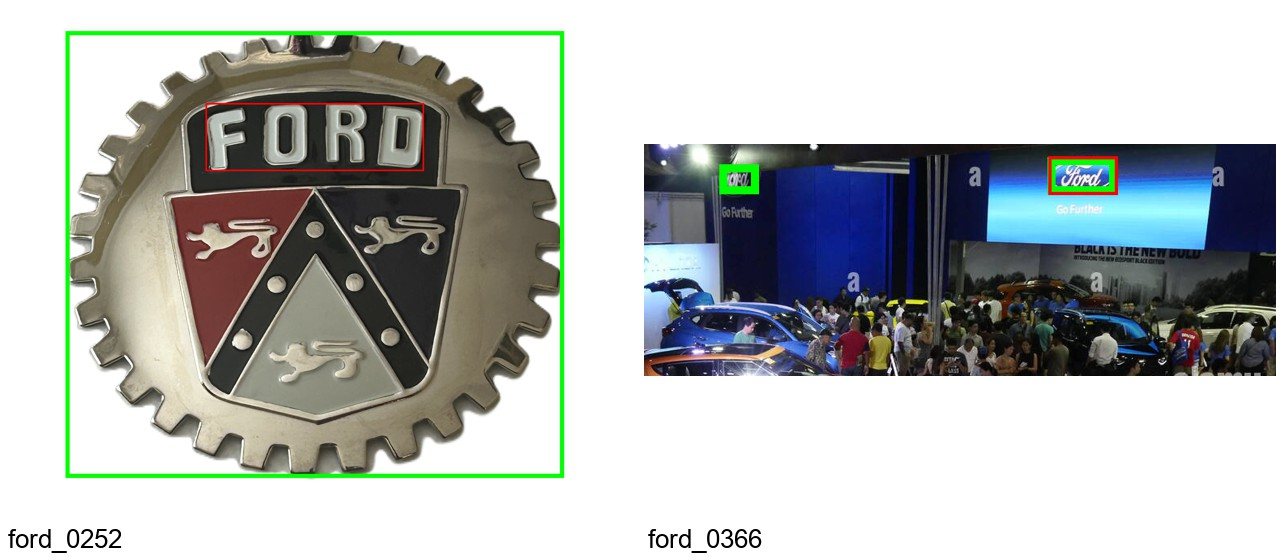
\includegraphics[width=\columnwidth]{tutarsizliklar.jpg}
\caption{Yeniden etiketlemede bulunan tutarsızlıklar (yeşil: ilk, kırmızı: ikinci etiketleme).}
\label{fig:relabel}
\end{figure}

\begin{figure*}[t]
\centering
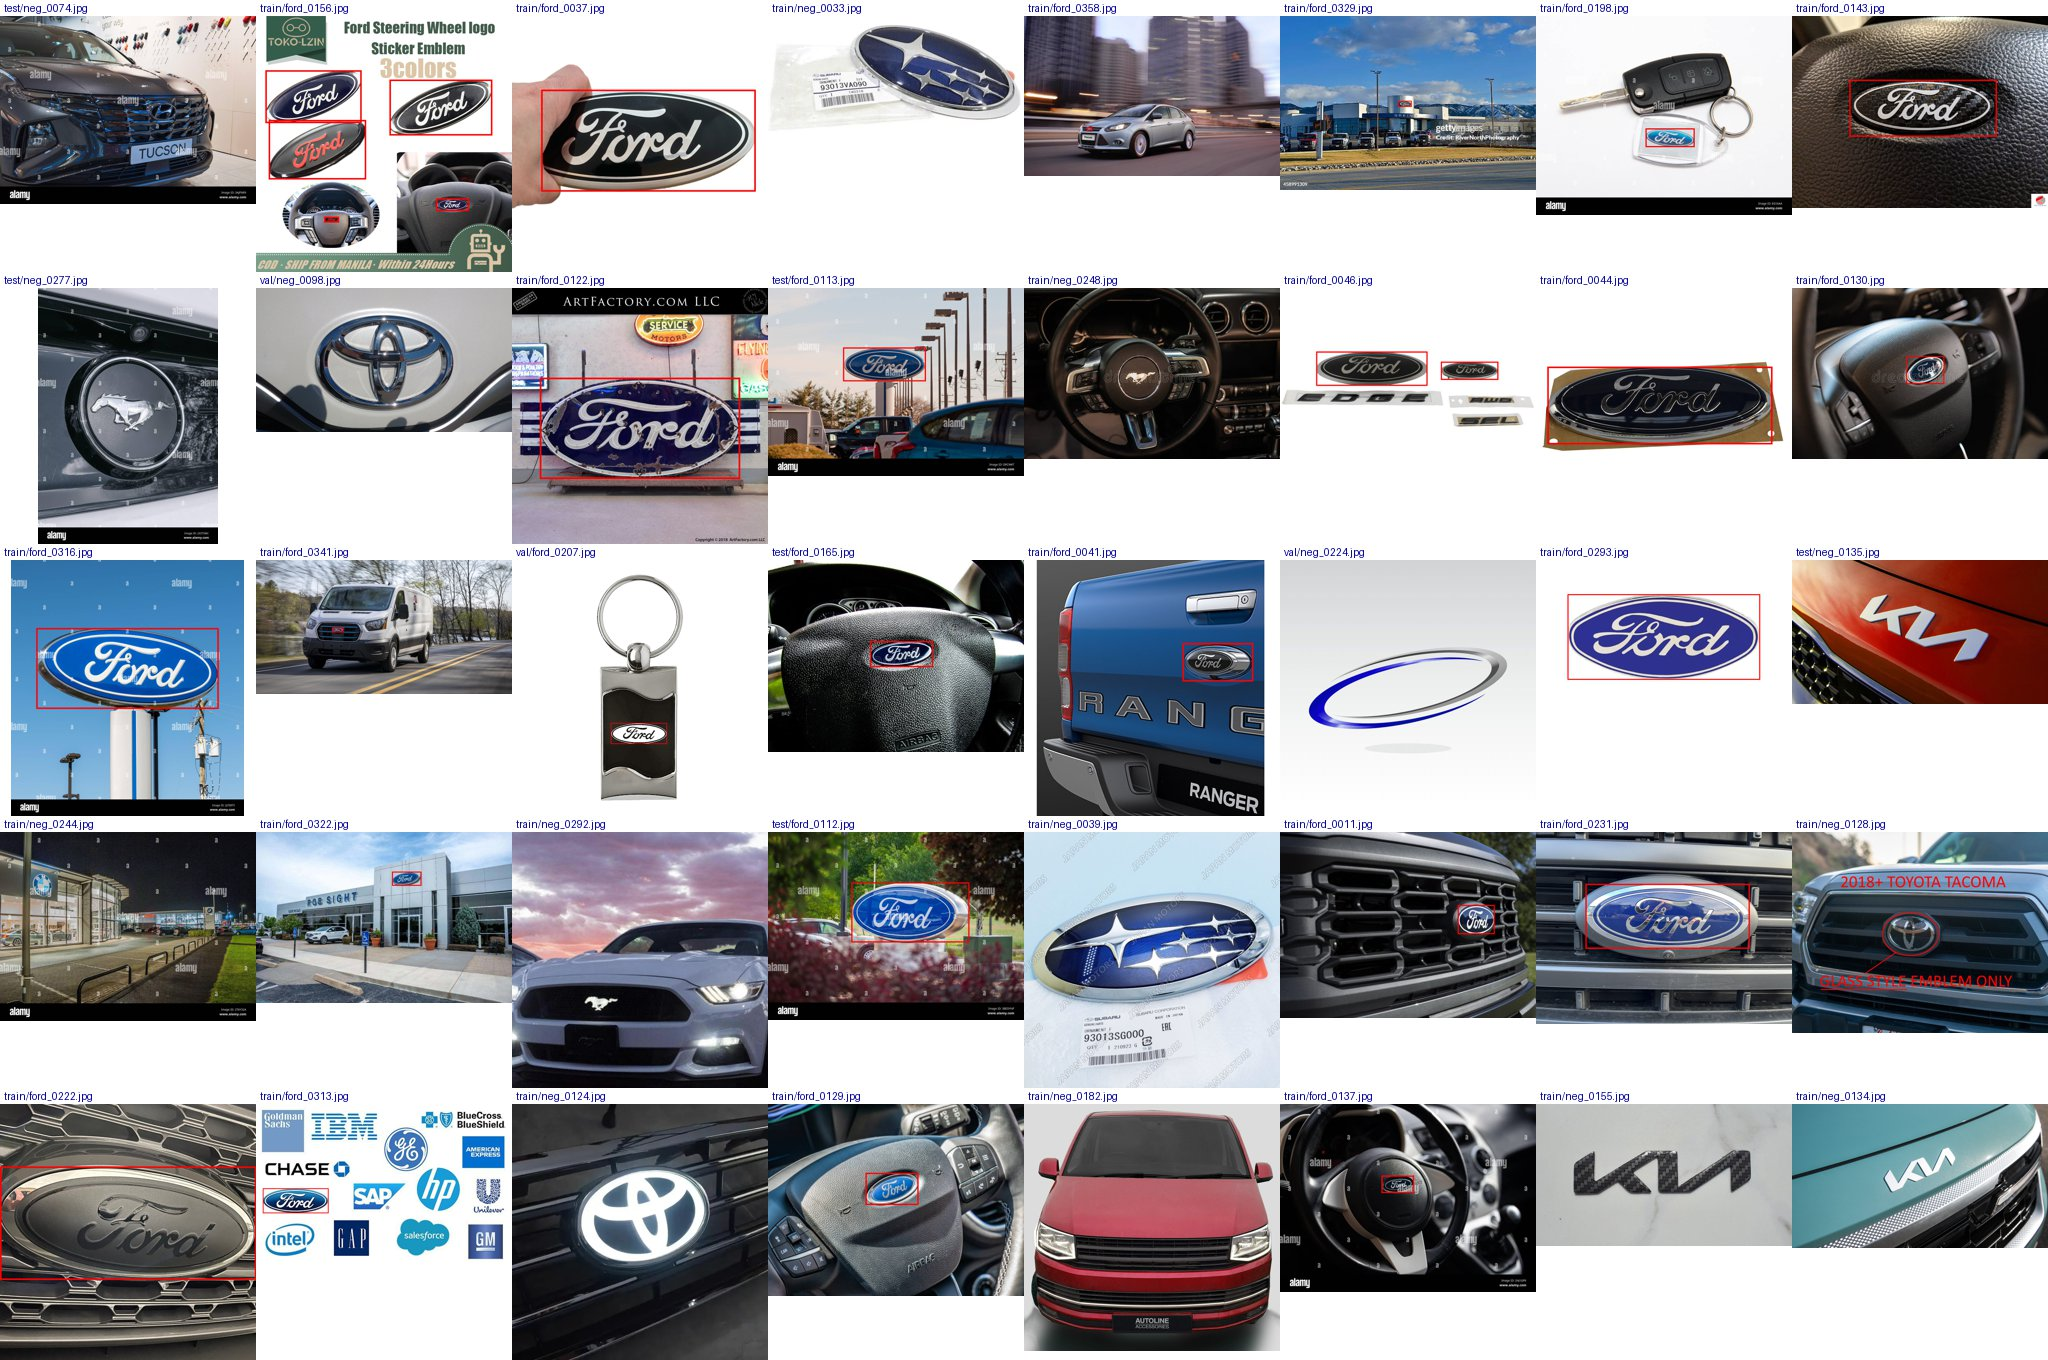
\includegraphics[width=\textwidth]{kalite_kontrol.jpg}
\caption{Kalite kontrol panosu: kutuları çizilmiş 40 rastgele görsel (seed 42).}
\label{fig:qc}
\end{figure*}

% ---------------------------------------------------------------------------
\section{Karşılaşılan Zorluklar ve Çözüm Önerileri}

\begin{itemize}
\item \textbf{Ham ve işlenmiş görsel uyuşmazlığı:} Roboflow'a ham görsellerin yüklenmesi
dosya adlarını ve görsel kümesini değiştirdi. pHash + en-boy oranı eşleştirmesiyle etiketler
yeniden etiketleme gerekmeden aktarıldı. \emph{Öneri:} Etiketleme aracına her zaman ön
işlenmiş ve son adlarını almış görseller yüklenmelidir.
\item \textbf{Arama sonuçlarındaki gürültü:} ``Ford Mustang'' gibi pozitif sorgular yalnızca
model rozeti içeren görseller, ``blue oval logos'' gibi negatif sorgular ise Ford logosu
içeren görseller döndürdü. Bunlar elle ayıklanıp doğru sınıfa aktarıldı; model rozetleri
değerli zor negatiflere dönüştü.
\item \textbf{Kural belirsizlikleri:} Eski armalar, oval içi yazı ve yazısız boş ovaller
etiketleyiciler arasında farklı yorumlanabiliyor. Bu durumlar özel karar olarak yazılı hale
getirildi. Yeniden etiketleme, belirsiz kuralların gerçek tutarsızlık ürettiğini gösterdi.
\item \textbf{Ölçek dengesizliği:} Web aramaları ağırlıklı olarak yakın çekim ürün
fotoğrafları döndürüyor. Hedefli bir küçük logo turuyla küçük kutu sayısı 19'dan 58'e
çıkarıldı, ancak bu sayı toplam kutuların hâlâ yaklaşık \%10'u. \emph{Öneri:} Video
karelerinden veya sokak görüntülerinden ek veri toplanabilir.
\item \textbf{Veri sızıntısı riski:} Aynı sahnenin farklı ajans kopyaları pHash $\le 4$
eşiğinin dışında kalabiliyor. Bölmede daha gevşek bir eşikle ($\le 10$) gruplama yapılarak bu
kopyalar aynı bölüme toplandı.
\item \textbf{Filigranlar ve kalabalık sahneler:} Stok fotoğraf filigranları ve düşük
kontrastlı tabelalar etiketlemeyi zorlaştırıyor; fuar görselinde bir logo ikinci etiketlemede
gözden kaçtı. \emph{Öneri:} Kalabalık sahnelerde yakınlaştırarak ikinci bir tarama
yapılmalıdır.
\end{itemize}

% ---------------------------------------------------------------------------
\section{Öğrenilen Dersler}

\begin{itemize}
\item Etiketleme kuralları başlangıçta ne kadar açık görünse de gerçek veride sınır durumlar
ortaya çıkıyor. Bu durumlar yazılı özel kararlara dönüştürülmeli ve tüm veri setine geriye
dönük uygulanmalıdır.
\item Tek bir yeniden etiketleme bulgusu sistematik bir hatayı ortaya çıkarabilir. ford\_0252
tutarsızlığı, aynı türdeki tüm armaların taranmasını sağladı.
\item Kalite kontrol için kutuları çizmek vazgeçilmezdir. Biçim hataları ve yanlış sınıf
atamaları sayısal kontrollerle değil, görsel incelemeyle bulundu.
\item Tüm adımların betikle ve sabit tohumla yapılması, yeni bir veri turu eklendiğinde veri
setinin tamamının dakikalar içinde ve aynı sonuçla yeniden üretilmesini sağladı.
\item Veri bölmede rastgelelik yeterli değildir; benzer görseller gruplanmazsa test başarımı
iyimser ölçülür.
\end{itemize}

% ---------------------------------------------------------------------------
\section{Sonuç}

Bu çalışmada 699 görsel ve 561 kutudan oluşan, zor negatiflerle desteklenmiş, grup korumalı
olarak bölünmüş ve YOLO ile COCO formatlarında sunulan bir Ford logosu veri seti
oluşturulmuştur. Veri seti yönergedeki tüm biçim kontrollerinden hatasız geçmekte ve
yeniden etiketleme ile ölçülen tutarlılığı yüksektir (ortalama IoU 0.971). Veri seti,
sonraki ödevlerde nesne tespiti ve logo var/yok sınıflandırması için doğrudan
kullanılacaktır.

\begin{thebibliography}{9}

\bibitem{yolov8}
G. Jocher, A. Chaurasia ve J. Qiu, ``Ultralytics YOLOv8,'' 2023. [Çevrimiçi].
Erişim: \url{https://github.com/ultralytics/ultralytics}

\bibitem{coco}
T.-Y. Lin \emph{vd.}, ``Microsoft COCO: Common objects in context,'' \emph{Proc. European
Conference on Computer Vision (ECCV)}, 2014, ss. 740--755.

\bibitem{icrawler}
K. Chen, ``icrawler: A multi-thread crawler framework,'' [Çevrimiçi].
Erişim: \url{https://github.com/hellock/icrawler}

\bibitem{imagehash}
J. Buchner, ``ImageHash: A Python perceptual image hashing module,'' [Çevrimiçi].
Erişim: \url{https://github.com/JohannesBuchner/imagehash}

\bibitem{roboflow}
Roboflow, ``Roboflow Annotate,'' [Çevrimiçi]. Erişim: \url{https://roboflow.com}

\bibitem{albumentations}
A. Buslaev \emph{vd.}, ``Albumentations: Fast and flexible image augmentations,''
\emph{Information}, c. 11, sy. 2, s. 125, 2020.

\end{thebibliography}

\end{document}
